\section{Introdução}

\begin{frame}{Contexto e Definição das RSSF}
    \begin{columns}
        \begin{column}{0.65\textwidth}
            \begin{itemize}
                \item Com o avanço da microeletrônica, os sistemas tradicionais cabeados e via satélite estão sendo substituídos por soluções mais ágeis e distribuídas.   
                \item As Redes de Sensores Sem Fio (RSSF) utilizam nós minúsculos e autônomos para monitorar grandezas específicas, como temperatura e luminosidade, em áreas de difícil acesso.   
                \item A principal vantagem dessa tecnologia é a escalabilidade, permitindo que centenas ou milhares de dispositivos formem malhas de sensoriamento de baixo custo em cidades inteligentes e indústrias.   
            \end{itemize}
        \end{column}
        
        \begin{column}{0.35\textwidth}
            \begin{figure}
                \centering
                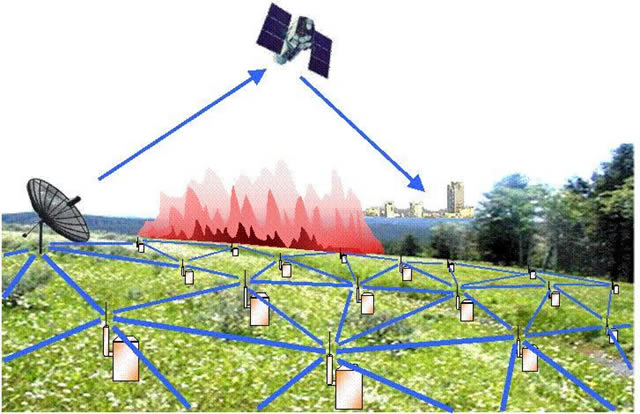
\includegraphics[width=\textwidth]{figuras/rede.jpg}
                \caption{Representação de uma RSSF.}
                \vspace{0.1cm}
                {\footnotesize Fonte: Pplware (sapo.pt)}
            \end{figure}
        \end{column}
    \end{columns}
\end{frame}

\begin{frame}{Desafios Energéticos e Resiliência}
    \begin{itemize}
        \item A operação em ambientes hostis gera restrições significativas, exigindo que os nós sensores otimizem seus escassos recursos energéticos através do processamento local de dados.   
        \item Em situações de falha (como esgotamento de bateria ou dano físico a um dispositivo), a rede precisa se reorganizar dinamicamente para garantir que o fluxo de informações não seja interrompido.   
        \item Para aumentar a sobrevida, a malha atua como um organismo reativo: os sensores permanecem em dormência profunda e despertam apenas para eventos ou alertas específicos.   
    \end{itemize}
\end{frame}

\begin{frame}{Indústria 4.0 e Objetivos do Trabalho}
    \begin{itemize}
        \item No cenário da Indústria 4.0, a conectividade distribuída dessas redes elimina cabeamentos complexos e viabiliza sistemas avançados de manutenção preditiva no chão de fábrica.   
    \end{itemize}
    
    \vspace{0.5cm}
    
    \begin{block}{Objetivo da Pesquisa}
        Apresentar os fundamentos das RSSF, detalhando suas aplicações práticas, os desafios operacionais das camadas físicas, as diretrizes de segurança cibernética e a evolução da infraestrutura com o uso da Inteligência Artificial.   
    \end{block}
\end{frame}